\documentclass{beamer}
\usepackage[english,russian]{babel}
\usepackage[utf8]{inputenc}
\usepackage{listings}
\usepackage{color}
\usepackage{xcolor}
\usepackage{ucs}
\lstset{inputencoding=utf8x, extendedchars=\true, captionpos=b, tabsize=3, keywordstyle=\color{blue},commentstyle=\color{green}, stringstyle=\color{red}, showstringspaces=false, basicstyle=\footnotesize,emph={label}, texcl}
%\lstset{texcl}
%\lstset{extendedchars=\true}
\lstset{
literate={а}{{\selectfont\char224}}1
{б}{{\selectfont\char225}}1
{в}{{\selectfont\char226}}1
{г}{{\selectfont\char227}}1
{д}{{\selectfont\char228}}1
{е}{{\selectfont\char229}}1
{ё}{{\"e}}1
{ж}{{\selectfont\char230}}1
{з}{{\selectfont\char231}}1
{и}{{\selectfont\char232}}1
{й}{{\selectfont\char233}}1
{к}{{\selectfont\char234}}1
{л}{{\selectfont\char235}}1
{м}{{\selectfont\char236}}1
{н}{{\selectfont\char237}}1
{о}{{\selectfont\char238}}1
{п}{{\selectfont\char239}}1
{р}{{\selectfont\char240}}1
{с}{{\selectfont\char241}}1
{т}{{\selectfont\char242}}1
{у}{{\selectfont\char243}}1
{ф}{{\selectfont\char244}}1
{х}{{\selectfont\char245}}1
{ц}{{\selectfont\char246}}1
{ч}{{\selectfont\char247}}1
{ш}{{\selectfont\char248}}1
{щ}{{\selectfont\char249}}1
{ъ}{{\selectfont\char250}}1
{ы}{{\selectfont\char251}}1
{ь}{{\selectfont\char252}}1
{э}{{\selectfont\char253}}1
{ю}{{\selectfont\char254}}1
{я}{{\selectfont\char255}}1
{А}{{\selectfont\char192}}1
{Б}{{\selectfont\char193}}1
{В}{{\selectfont\char194}}1
{Г}{{\selectfont\char195}}1
{Д}{{\selectfont\char196}}1
{Е}{{\selectfont\char197}}1
{Ё}{{\"E}}1
{Ж}{{\selectfont\char198}}1
{З}{{\selectfont\char199}}1
{И}{{\selectfont\char200}}1
{Й}{{\selectfont\char201}}1
{К}{{\selectfont\char202}}1
{Л}{{\selectfont\char203}}1
{М}{{\selectfont\char204}}1
{Н}{{\selectfont\char205}}1
{О}{{\selectfont\char206}}1
{П}{{\selectfont\char207}}1
{Р}{{\selectfont\char208}}1
{С}{{\selectfont\char209}}1
{Т}{{\selectfont\char210}}1
{У}{{\selectfont\char211}}1
{Ф}{{\selectfont\char212}}1
{Х}{{\selectfont\char213}}1
{Ц}{{\selectfont\char214}}1
{Ч}{{\selectfont\char215}}1
{Ш}{{\selectfont\char216}}1
{Щ}{{\selectfont\char217}}1
{Ъ}{{\selectfont\char218}}1
{Ы}{{\selectfont\char219}}1
{Ь}{{\selectfont\char220}}1
{Э}{{\selectfont\char221}}1
{Ю}{{\selectfont\char222}}1
{Я}{{\selectfont\char223}}1
}
% Стиль презентации
\usetheme{Madrid}
\begin{document}
\title{Квантовые языки программирования}  
\author[Донцов А.]{Донцов Александр\inst{1}, 571 гр.}

\institute[АлтГУ]
{	\inst{1}%
ГОУ ВПО <<Алтайский государственный университет>>\\
Кафедра радиофизики и теоретической физики
}

\date{
   Барнаул\\
    2011г.
}
\begin{frame}
\begin{block}{}
\begin{center}
ФГБОУ ВПО <<Алтайский государственный университет>>\\
Физико-технический факультет\\
Кафедра радиофизики и теоретической физики
\end{center}
\end{block}
  \begin{columns}
    \column{.9\textwidth}
      \begin{block}{}
	\begin{flushleft}
	  {{\Large \bf Квантовые алгоритмы и языки программирования\\}}
	\end{flushleft}
      \end{block}
    \column{.1\textwidth}
  \end{columns}
\begin{center}
\textbf{Донцов Александр Андреевич}
\end{center}
  \begin{columns}
    \column{.8\textwidth}
      \begin{flushright}
      \end{flushright}
    \column{.2\textwidth}
  \end{columns}

  \begin{columns}
    \column{.1\textwidth}
    \column{.9\textwidth}
      \begin{flushright}
	Научный руководитель: к.ф.-м.н. Н.\,В. Волков\\
      \end{flushright}
  \end{columns}
\end{frame}
\begin{frame}
 \frametitle{Актуальность}
Важным направление в исследовании вычислительных устройств, основанных на квантовых эффектах,  является компьютерное моделирование.  Многие квантовые алгоритмы были разработаны совсем недавно или же разрабатываются в настоящее время. И возникают вполне естественные вопросы:
  
\begin{itemize}
  \item Как проверить, что они действительно работают? 
 
  \item Существуют какие-либо ограничения? 

  \item Действительно ли они эффективны? 
\end{itemize}
Компьютерное моделирование должно помочь с ответами на эти вопросы. 
\end{frame}
\begin{frame}
\frametitle{Описание квантового алгоритма}
\begin{block}{Описание квантового алгоритма}
Наиболее популярны три способа описания квантового алгоритма:
\begin{itemize}
  \item Описание в виде квантовой схемы.
  \item Описание в виде квантовой машины Тьюринга.
  \item Описание в виде программы на некотором, специализированном языке программирования.
\end{itemize}
\end{block}
\end{frame}
\begin{frame}
 \frametitle{}
 \begin{block}{Представление квантовых вычеслений}
 Существующее программное обеспечение для моделирования квантовых вычислений можно классифицировать следующим
образом:
По объекту моделирования:
\begin{itemize}
  \item Программное обеспечение, моделирующее поведение квантовой системы,путем решения уравнения Шредингера. Такие программы называют эмуляторами.
  \item Программное обеспечение, моделирующее абстрактную математическую модель квантового компьютера. Такие программы называют симуляторами (simulators).
\end{itemize}
\end{block}
\end{frame}
\begin{frame}
 \frametitle{Архитектура}
\begin{figure}[h]
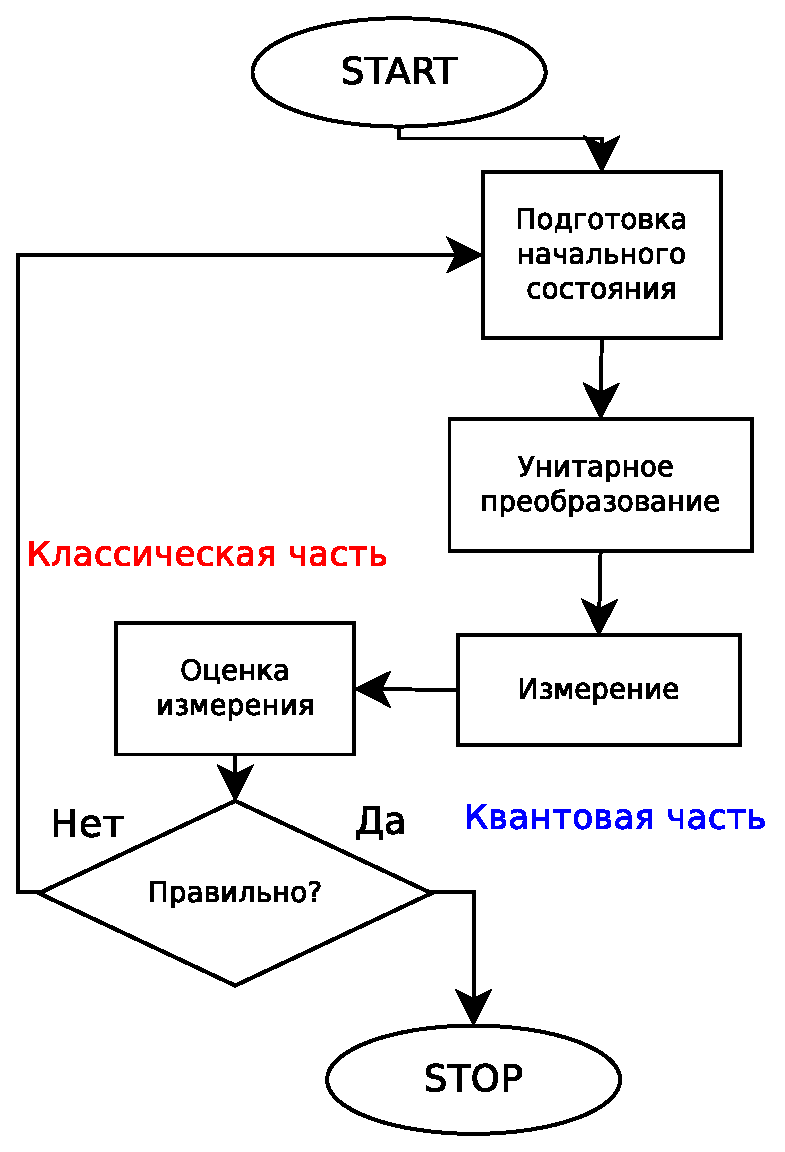
\includegraphics[width=0.42\linewidth]{images/kk1.eps}
\caption{Схема устройства квантового компьютера}
\end{figure} 
\end{frame}
\begin{frame}
 \frametitle{Язык квантового программирования QCL}
 \begin{block}{История}
 QCL является императивным языком квантового программирования, создатель Bernhard Ömer, сотрудник Австрийского Технологического института, QCL реализован на C++. QCL - один из первых квантовых языков программирования и один из наиболее развитых. Первая версия вышла в 2003 году, на сегодняшний день последней версией является 0.6.3. QCL позволяет сочетать в одной программе, как классический, так и квантовый код. Является свободным программным обеспечением, распространяется под лицензией GPL.
\end{block}
\end{frame}

\begin{frame}[fragile]
 \frametitle{Язык квантового программирования QCL}
 \begin{block}{Основные понятия}
 \begin{itemize}
%  \item \begin{lstlisting} qcl> qureg x[1] //  Кубит - квантовый регистр единичной длины. \end{lstlisting}
  \item \verb|qcl> qureg x[1]| //  Кубит --- квантовый регистр единичной длины.
  \item procedure - Классические процедуры контроля
  \item operator - Унитарные операторы
  \item qufunct - Квантовые функции
  \item functions - Математические функции
 \end{itemize}
 \end{block}
\end{frame}


\begin{frame}[fragile]
 \frametitle{Реализация квантового преобразования Фурье}
 \begin{block}{Подготовка регистра}
 \begin{verbatim}
cond qufunct flip(qureg q) { 
  int i;                // Объявление счётчика цикла
  for i=0 to #q/2-1 {   // swap 2 симметричных бита
    Swap(q[i],q[#q-i-1]);
  }
}
\end{verbatim}  
 \end{block}
\end{frame}

\begin{frame}[fragile]
 \frametitle{Реализация квантового преобразования Фурье}
 \begin{block}{Подготовка регистра}
 \begin{verbatim}
 operator dft(qureg q) { // main operator
  const n=#q;           // n равно длине регистра q
  int i; int j;         // объявляем сётчики циклов
  for i=1 to n {
    for j=1 to i-1 {    // перебор и по условию поворот фазы
      V(pi/2^(i-j),q[n-i] & q[n-j]);
//      if q[n-i] and q[n-j] { Phase(pi/2^(i-j)); }
    }
    H(q[n-i]);          // qubit rotation
  }    
  flip(q);              // swap bit order of the output
}

set library 0;
\end{verbatim}  
 \end{block}
\end{frame}

\begin{frame}
 \frametitle{Результаты}

\begin{itemize}
  \item Обзор электронных и печатных ресурсов по современным языкам программирования для симуляции квантовых вычислений. Сравнительная характеристика имеющихся языков.
  \item Изучение синтаксисов языков квантового программирования.
  \item Реализация квантовых схем.
\end{itemize}
\end{frame}


\end{document}